\documentclass{article}
\usepackage{amsmath}
\usepackage{algorithm}
\usepackage[noend]{algpseudocode}
\usepackage{ dsfont }
\usepackage{amssymb}
\usepackage{setspace}
\usepackage{graphicx}
\usepackage{subcaption}

% Questa linea raddoppia lo spazio tra una riga e l'altra per tutto il documento %
\doublespacing

\begin{document}
% Abstract %
\thispagestyle{plain}
\begin{center}
    \Large
    \textbf{Computational Mathematics for Learning and Data Analysis}

    \vspace{0.4cm}
    \large
    2019 / 2020

    \vspace{0.4cm}
    \textbf{Poggiali Alessandro, Berti Stefano}

    \vspace{0.9cm}
\end{center}

% Nuova pagina %
\newpage
% Setting the stage %
\section{Setting the stage}\label{sec:setting-the-stage}

\subsection{The problem: Least Squares}\label{subsec:linear-square-problem}
Our problem is to find an array x such that \\\\
\centerline{$\min_{x \in \mathds{R}^n}\|Ax-b\|$} \\\\
holds, where
\begin{itemize}
	\item $A$ is a \textit{tall thin matrix} (so it is a matrix $A\in M(m, n, R)$ where $m \gg n$)
	\item $b$ is a vector of real number
	\item $\|.\|$ is the \textit{2-norm} or \textit{Euclidean Norm}: $\|x\| := \sqrt{\sum_{i=1}^n x_i}$
\end{itemize}
and so to find the closest vector to $b$ inside the hyperplane $Im(A)$.

% Conjugate gradiend method %
\subsection{First algorithm: Conjugate Gradient Method}\label{subsec:conjugate-gradient-method}
In general, if a square matrix $B = B^{T}$ is positive definite, then we can find a solution to $Bx = c$ by minimizing the (strictly convex) function 
\begin{equation}\label{eq:cgfunction}
f(x) = \frac{1}{2}x^{T}Bx - c^{T}x  
\end{equation}
(that is equal to set $\nabla f(x) = Bx - c = 0$). However our matrix $A$ is a \emph{tall thin matrix} and since in this case finding a solution to  $Ax = b$ is equivalent to solving the normal equations
\[
A^{T}Ax - A^{T}b = 0
\]
then we can use \textit{Conjugate gradient} method to minimize the function
\[
f(x) = \frac{1}{2}x^{T}A^{T}Ax - x^{T}A^{T}b
\]
From now on we set $B = A^{T}A$ and $c = A^{T}b$ so our function to minimize become exactly the (\ref{eq:cgfunction}), where $B$ is positive definite. 
\\We remember that \begin{itemize}
\item \textbf{B-orthogonal}: $x, y \in R^{m}$ are B-orthogonal if $x^{T}By = 0$
\item \textbf{B-norm}: the B-norm of $x \in R^{m}$ is $\|x\|_{B} := (x^{t}Bx)^{\frac{1}{2}}$. Note that if B is \textit{positive definite}, then the B-norm is $\geq 0$ (it is $0$ only for the $0$ vector)
\end{itemize}
Let $x_{k}$ be the parameter vector after the $k$-th iteration, then the residual vector is $r_{k} = b - Ax_{k}$ and the negative gradient $g_{k} = -\nabla f(x_{k}) = c - Bx = A^{T}b - A^{T}Ax = A^{T}r_{k}$. The step size $\alpha_{k}$ can be computed in a similar way as in the standard CG method, but here the denominator is $d_{k}^{T}Bd_k= d_{k}^{T}A^{T}Ad_k = \|Ad_{k}\|^2$ and so it can be obtained without calculating $B = A^{T}A$.
\\To update the residual, we use the fact that $r_{k} = b - Ax_{k} = [x_{k} = x_{k-1} + \alpha_{k-1}d_{k-1}] = b - A(x_{k-1} + \alpha_{k-1}d_{k-1}) = [b-Ax_{k-1} = r_{k-1}] = r_{k-1} - \alpha_{k-1}Ad_{k-1}$. The trick about conjugate gradient is that at each step we generate a new search direction, which is not exactly the residual, but is the residual modified to be $B$-orthogonal to the previous search direction. In this way, $\beta_{k}$ is a scalar that is chosen s.t. $d_{k}$ is $B$-orthogonal to $d_{k-1}$.

% QR factorization method %
\subsection{Second algorithm: QR factorization with Householder Reflectors}\label{subsec:qr-factorization-with-householder-reflectors}
To solve the Least Square Problem, we use the \textit{thin QR factorization} with all the optimization seen (fast Householder-vector product, cancellation problem resolution, manually changing known entries) in order to factorize $A$ as $Q_{1}R_{1}$.
We use a variant \cite{nla} of the \textit{thin QR factorization} where we do not form the matrix $Q$, but we keep the Householder vector $u_{k}$ to perform implicit product with $Q$ and $Q^{T}$.
With this factorization, we can write $\|Ax - b\|$ as $\left\lVert \begin{bmatrix} R_{1}x - Q_{1}^{T}b \\ Q_{2}^{T}b\end{bmatrix} \right\lVert$
and now we can chose $x$ such that $R_{1}x - Q_{1}^{T}b = 0$, which is $x = R_{1}^{-1}Q_{1}^{T}b$ (if $R_{1}$ is invertible).
We can write $x = R^{-1}(Q^{T}b) = R^{-1}(((I-2v_{1}v_{1}^{T})(I-2v_{2}v_{2}^{T})\dots(I-2v_{m}v_{m}^{T}))^{T}b)$
Finally we should have $x  = \arg\!\min_{x \in  \mathds{R}^n}\|Ax - b\| = R_{1}^{-1}Q_{1}^{T}b$ and $\|Ax - b\| = \|Q_{2}^{T}b\|$.

\section{What to expect from the algorithms}\label{sec:what-to-expect-from-the-algorithms}

\subsection{Conjugate Gradient}\label{subsec:conjugate-gradient}
Our system $Ax = b$ is equivalent to the system $Bx = c$, where $B = A^{T}A$ is symmetric and positive definite and $c = A^{T}b$. However, from a numerical point of view, the two systems are different, because of rounding-off errors that occur in joining the product $A^{T}A$. But since our algorithm does not involve the computation of $B = A^{T}A$, then we have the same convergence result as in the standard CG method. In particular we know that this method gives the solution in $n$ steps if no rounding-off error occurs, where $n$ is the size of $B$, namely the smallest size of our original rectangular matrix $A$. In realistic cases, the absence of rounding-off errors cannot be assured and so we need more than $n$ step or even to restart the algorithm many times. Also the basic relations concerning convergence ($<r_i,r_k>\,= 0, <Ad_i,d_k>\,= 0$ for $i \ne k$) will not be satisfied exactly and therefore $x_n$ will not be as good an estimate the exact solution as desired. From \cite{hestenes1952methods} follows that the larger the ratios $\alpha_i / \alpha_{i-1}$, the more rapidily the rounding-off errors accumulate. Moreover, since $\alpha_i$ lie on the range
\[
1 / \lambda_{max} < \alpha_i < 1 / \lambda_{min}
\] 
the ratio $\rho = \lambda_{max}/\lambda_{min}$ gives us an upper bound of the critical ratio  $\alpha_i / \alpha_{i-1}$ which determines the stability of the entire process. So we would like to have $\rho$ near one, that means our matrix is near multiple of the identity and then the CG method is relatively stable. 

The algorithm performs at every step two multiplications  (one is enough if we compute it and store it) of $A$ with the $n$-vector $d_i$ $(O(mn))$ and one multiplication of $A^{T}$ with the $m$-vector $r_i$ $(O(nm))$. 
So, the total cost is $n(O(mn) + O((nm)) + O(n)) \approx O(n^2m)$, where $O(n)$ comes from the scalars product between $n$-vectors to compute the norms for every steps.

The convergence of the Conjugate Gradient Method depends on the maximum eigenvalue $\lambda_{max}$ and the minimum eigenvalue $\lambda_{min}$, and CG converges with rate 
\begin{equation}\label{eq:cgconv}
\|x-x_{k}\| \leq \left\lVert\frac{\sqrt{\lambda_{max}}-\sqrt{\lambda_{min}}}{\sqrt{\lambda_{max}}+\sqrt{\lambda_{min}}}\right\rVert^{k}  \|x - x_{0}\| 
\end{equation}

\subsection{QR with HouseHolder}\label{subsec:qr-with-householder}
The QR factorization has a cancellation problem during the Householder reflector construction that is easily fixed by summing first entry and norm instead of subtract it.
\\Apart from that, since every step is \textit{backward stable}, the factorization algorithm is \textit{backward stable}: the computed $Q$, $R$ are the exact result of $qr(A + \Delta A)$ where $ \left\lVert \Delta A \right\rVert \leq O(u)\left\lVert A \right\rVert$, so we only have intrinsic representation errors.
\\By looking at the residual $\left\lVert A x - b\right\rVert$, we can't say if our computed $x$ is close to the true solution $x^{*}$: the residual can be arbitrarily large because it depends on the problem.
The computed $x$ solves the modified problem $\min \left\lVert Ax - (b + Q_{1}r)\right\rVert$, and $x$ is close to the true solution $x^{*}$ if the residual of the top block $r_{1} = Q_{1}^{T}(Ax - b)$ is close to 0.
Moreover, $\frac{\left\lVert x - x^{*} \right\rVert}{ \left\lVert x^{*} \right\rVert} \leq k_{rel, b\rightarrow x}\frac{\left\lVert r \right\rVert}{\left\lVert b \right\rVert}$.
\\The computational cost for thin QR factorization is $2mn^2 - \frac{2}{3}n^3 + O(mn)$ flops, which represents two cases: if $m \approx n$, we have that the cost is $\frac{4}{3}n^3$, if $m \gg n$ the cost scales like $2mn^2$, so it scales linearly with respect to the biggest dimension of A .
\\Before we said that $x = R_{1}^{-1}Q_{1}^{T}b$, but to be able to calculate it we need $R_{1}$ to be invertible.
We know that $A$ has full column rank $\iff Az \neq 0 \forall z \neq 0 \iff z^{T}A^{T}Az = \left\lVert Az \right\rVert^{2} \forall z \neq 0 \iff A^{T}A$ is positive definite $\iff$ all eigenvalues of $A^{T}A$ are $> 0\iff $0 is not an eigenvalue of $A^{T}A \iff A^{T}A = (Q_{1}R_{1})^{T}Q_{1}R_{1} = R_{1}^{T}Q_{1}^{T}Q_{1}R_{1} = R_{1}^{T}R_{1}$ is invertible $\iff det(A^{T}A) = det(R_{1}^{T})det(R_{1}) \neq 0 \iff det(R_{1}) \neq 0 \iff R_{1}$ is invertible.
So if $A$ has full column rank, $\min_{x \in \mathds{R}^n}\|Ax-b\|$ has solution and it is unique.
$R_{1}$ is invertible also if all elements on its diagonal are $\neq 0$.
\\The cost to solve $x = R_{1}^{-1}(Q_{1}^{T})b$ is a multiplication $c = (Q_{1}^{T})b$, which costs $O(mn)$, and the resolution of the triangular system $R_{1}x = c$ with back-substitution, which costs $O(n^{2})$.
Anyway, the overall cost $O(mn) + O(n^{2})$ is negligible with respect to the cost $O(mn^{2})$ to compute $Q_{1}, R_{1}$.
This factorization algorithm is bandwidth heavy and not parallelizable, as every reflection that produces a new zero element changes the entirety of both Q and R matrices

\section{Input data}\label{sec:input-data}
Our input data is the matrix A, which is the tall thin matrix used as input in the \textit{ML-cup 2019--2020} competition.
Its shape is $(1765, 20)$, we augmented it with few functions of the features of the dataset:
\begin{itemize}
	\item \textbf{21\textsuperscript{th} column}: logarithm of the absolute value of the 1\textsuperscript{st} column
	\item \textbf{22\textsuperscript{th} column}: product of 2\textsuperscript{nd}, 3\textsuperscript{rd} and 4\textsuperscript{th} columns
	\item \textbf{23\textsuperscript{th} column}: 5\textsuperscript{th} column to square
\end{itemize}
So the final shape of $A$ is $(1765, 23)$.
    The condition number of the matrix $A$ (calculated with \textit{numpy.linalg.cond}, which does SVD and $\frac{\sigma_{1}}{\sigma_{n}}$) is $\approx 400000 (4 \times 10^{5})$, while the condition number of a random matrix with the same dimension and same range of values (min and max of the 2 matrices are the same) is $\approx 1.7$.
    We can conclude that the matrix $A$ is ill conditioned, so it is almost singular and the solution of our problem could be not accurate.
    Anyway, we know that the solution of the least square problem exists and it is unique, because $A$ is a full column rank matrix ($rank(A) = n = 23$), where rank is calculated as the number of singular values $> \max(\sigma_{i}) \times max(m, n) \times eps$, which is the same approach used in MATLAB .

\section{Code}\label{sec:code}
The code has been implemented in \textit{Python}, we used \textit{Numpy} for array manipulation.
\subsection{Conjugate gradient method Code}
The Algorithm 1 performs the CG method applied to our function \ref{eq:cgfunction}, starting from an initial guess of $x$. For each iteration we store the pruduct $Ad_k$ in a variable so that it can be computed only once insted of twice.
% CG pseudocode
\makeatletter
\makeatother
\begin{algorithm}
\caption{LS resolution with CG method}
\begin{algorithmic}[1]
\Function{$x \gets A, b$}{}
\State $x_0 \gets starting\,guess$
\State $r_0 \gets b -  Ax_0$
\State $g_0 \gets A^{T}r_0$ 
\State \emph{for i = 1:m}:
\State \quad\emph{if $g_{k-1} = 0$}:
\State\quad\quad\textit{return $x_{k-1}$}
\State \quad\emph{if $i > 1$}:
\State\quad\quad{$\beta_{k} = - \|g_{k-1}\|^2 / \|g_{k-2}\|^2$}
\State \quad\emph{if $i = 1$}: 
\State\quad\quad{$d_{k} = g_{0}$}
\State \quad\emph{else}: 
\State\quad\quad{$d_{k} = g_{k-1} - \beta_{k}d_{k-1}$}
\State\quad $\alpha_{k} = \|g_{k-1}\|^2 / \|Ad_{k}\|^2$
\State\quad $x_{k} = x_{k-1} + \alpha_{k}d_{k}$
\State\quad $r_{k} = r_{k-1} - \alpha_{k}Ad_{k}$
\State\quad $g_{k} = A^{T}r_{k}$
\State\textit{return $x_{m}$}
\EndFunction
\end{algorithmic}
\end{algorithm}
\subsection{QR factorization method code}\label{subsec:qr-code}
In line 6 of Algorithm 4, we used \textit{scipy.linalg.solve\_triangular} to compute the solution of the linear system $R_{1}x = Q_{1}^{T}b$ by back-substitution, where $Q_{1}^{T}b$ is the vector computed by implicit product.
 % Householder reflector pseudocode
\makeatletter
\def\BState{\State\hskip-\ALG@thistlm}
\makeatother
\begin{algorithm}
\caption{Householder reflector}
\begin{algorithmic}[1]
\Function{$[v, s] \gets householder\_vector(x)$}{}
\State $s \gets -sign(x[0]) \times norm(x)$
\State $v \gets x$
\State $v[0] \gets v[0] -s$
\State $v \gets \frac{v}{norm(v)}$
\State \textit{return v, s}
\EndFunction
\end{algorithmic}
\end{algorithm}
% QR factorization pseudocode
\makeatletter
\makeatother
\begin{algorithm}
\caption{QR factorization with Householder Reflectors}
\begin{algorithmic}[1]
\Function{$[V, R] \gets qr\_factorization(A)$}{}
\BState \emph{top}:
\State $\textit{[m, n]} \gets \textit{size(A)}$
\State $\textit{V} \gets \textit{emptyList}$
\BState \emph{loop}:
\State \emph{for j = 1:min(m-1, n)}:
\State \quad$\textit{[v, s]} \gets \textit{householder\_vector(A(j:end, j))}$
\State \quad$\textit{A[j, j]} \gets \textit{s}$
\State \quad$\textit{A[j+1:end, j]} \gets \textit{0}$
\State \quad$\textit{A[j:end, j:end]} \gets \textit{A[j:end, j:end]} - 2\times v \times (v^{T} \times \textit{A[j:end, j+1:end])}$
\State \quad$\textit{V} \gets \textit{V.insert(v)}$
\BState \emph{end}:
\State $\textit{R = A}$
\State \textit{return V, R}
\EndFunction
\end{algorithmic}
\end{algorithm}
% Resolution pseudocode
\makeatletter
\makeatother
\begin{algorithm}
\caption{LS resolution with QR factorization}
\begin{algorithmic}[1]
\Function{$x \gets A, b$}{}
\State $\textit{[V, R]} \gets \textit{qr\_factorization(A)}$
\State $x \gets b$
\State \emph{for i = 1:n}:
\State \quad$x[i:end] \gets x[i:end] - 2 \times v_{i} \times (v_{i}^{T} \times x[i:end])$
\State $x \gets R^{-1}x$
\State \textit{return x}
\EndFunction
\end{algorithmic}
\end{algorithm}

\section{Experimental set up}\label{sec:experimental-set-up}
We are going to compare the two methods over the ML-cup in terms of time spent, memory usage and quality of the solution.
We will look how much our solutions are good in terms of residual and how much we got close to the true solution.
We will check the condition angle of the problem, to understand how much our solution is stable, and we will compare it with a random matrix with the same dimension and range of values of the ML-cup one.
Finally, we will test which is the maximum problem dimension computable for the two methods with a given RAM .
Moreover, for the QR factorization, we are going to test how the computational cost scales varying the dimension $m$ over the 3 matrices $m \times m$, $m \times n$ with $m > n$ and $m \times n$ with $m \gg n$.

\section{Results}\label{sec:results}
\begin{table}[h!]
    \begin{center}
        \caption{Results for ML-cup}
        \label{tab:table4}
        \begin{tabular}{l|c|c|c|c|r}
            \textbf{method} & \textbf{Time [ns]} & \textbf{Space [bytes]} & $\frac{\|\textbf{Ax - b}\|}{\left\lVert b \right\rVert}$ & $\|\textbf{A}^{T}(\textbf{Ax} - \textbf{b})\|$ & $\|\textbf{Q}^{T}\textbf{(Ax - b)}\|$\\
            \hline
            CG & 1557500 & 15040 & 0.4369 & 7.86e-03 & - \\
            QR & 5813172 & 322736 & 0.4369 & 1.4766e-07 & 1.6231e-09 \\
            np.linalg.qr & 1308946 & 328992 & 0.4369 & 2.3783e-07 & 1.6379e-09 \\
            scipy.linalg.qr & 7631518 & 328992 & 0.4369 & 2.5920e-07 & 1.7830e-09
        \end{tabular}
    \end{center}
\end{table}

\subsection{Time}\label{subsec:time}
For the time results we averaged 1000 run using \textit{time.monotonic\_ns()}, and we removed the best and worst 100 ones.
The CG method is $\sim 4$ times faster than the QR method: for the QR method we need n steps to compute the n $v_{i}$'s vector and the matrix $R$, while the CG method is an iterative method and we can choose after how many iterations to stop.
In Table \ref{tab:table4} we report the results obtained performing the CG method for $n$ iterations, since theoretically this algorithm should return the exact solution after $n$ steps.
However, after such a low number of iterations we fail to achieve a good accuracy.
Plots in Fiugre \ref{cg_acc} show how the number of iterations changes according to different levels of accuracy required by the algorithm.
The maximum level of accuracy reached by the CG method applied to our problem is $\approx 10^{-11}$ [figure \ref{cg_acc1}].
After that the rounding-off errors accomulate a lot and the algorithm no longer converges.
This is because our problem is ill conditioned.
In fact, if we execute the same approach to a random problem (random matrix $A$ and random vector $b$ with the same dimensions and the same ranges of values of our inputs) we note that [figure \ref{cg_acc2}] the number of iterations required to get the same accuracy is definitely lower.
These graphs show also that the convergence of the CG method is almost linear, as formula \eqref{eq:cgconv} states.
For what concerns the choice of the initial vector $x_0$ we used the 0 vector for all the experiments.
Since our function to minimize is a convex function, whatever starting point we choose the algorithm converges to the (unique) optimal solution.
In Figure \ref{cg_x0} we report in how many iterations the CG method converges to the optimal solution with a fixed level of accuracy ($10^{-11}$) with different starting point.
We note that if we start close to the optimal solution the algorithm requires few iterations while if we choose a starting vector far away from the optimum the number of iterations increases until it reaches a constant trend.
In fact, from \eqref{eq:cgconv} follows that the rate of convergence is determined by the distance between the initial vector and the optimal solution.
So it is preferable to start with an initial guess close to the optimum but since we don't have such estimate in advance, the 0 vector is a good trade-off.
\subsection{Space}\label{subsec:space}
With space we mean the additional number of bytes used by the methods in addition to the inputs, we measured it with \textit{numpy.array.nbytes}.
The space used by the QR method, if we assume that we don't want to preserve the input matrix A (that will become the upper triangular matrix R), is the number of bytes needed to save the n $v_{i}$'s vector of floats with length in [1765, 1743], and it is $\sim 1725 \times 23 \times 8$.
The computation to calculate x is done "in place", so no more space is required.
There is a little difference between the space used by our implementation and the one of numpy, because we don't form the matrix $Q$ of size $m \times n$, but we have $n$ vector of size $m, m-1, \dots, m-n$.
The CG method stores five $n$-vectors ($x, d, g, g_{i-1}$ and $g_{i-2}$) and one $m$-vector ($r$) for each iteration but since we don't need to keep whole ‘history’ we can rewrite them every time.
So the total space for CG is $(23\times5 + 1765)\times8 = 15040$.
If we assume to have a RAM of 4 GB and we fix $n$, we can compute the maximum computable dimension of m that we call $M$.
We obtain that, if $n=10$, $M_{QR} = 50 \times 10^{6}$ and $M_{CG}\sim 500 \times 10^{6} (499999950)$, and with $n=10000$, $M_{QR} = 50 \times 10^{3}$ and still $M_{CG} \sim 500\times 10^{6} (499950000)$.
The maximum dimension in case of square matrix $N$ is $N_{CG} = \frac{RAM}{48} = 500 \times 10^{9}$ and $N_{QR} = \sqrt{\frac{RAM}{8}} = 22360$.
We can conclude that the space needed by CG is $O(n+m)$, while the space needed by QR is $O(nm)$ for the general case.
For square matrices ($n=m$) the space needed by the CG is $O(n)$ and the space needed by the QR is $O(n^{2})$.
It turns out that the CG method is more suitable for large matrices in terms of space.

\subsection{Quality of solution}\label{subsec:quality-of-solution}
The angle $\theta$ between $Ax$ and $b$ is telling us how well we can approximate $b$ from $Ax$, and the bigger it is, the higher is the changing in the solution $x$ w.r.t a small change in $b$.
We compute it as $\arccos(\frac{\left\lVert Ax \right\rVert}{\left\lVert b \right\rVert})$, and its value is 0.45.
To understand if this value is big or not, we compared it with the one obtained with random inputs $A$ and $b$ with same dimensions and range of values, and we obtained 0.82, so this value doesn't seem to be such big.
Anyway, the condition number of the matrix A is big ($k(A) \sim 400000$), and if we compute the condition number w.r.t input b we obtain $k_{rel, b\rightarrow x} \leq \frac{k(A)}{\cos(\theta)} \sim 450000$ and w.r.t input A we obtain $k_{rel, A \rightarrow x} \leq k(A) + k(A)^{2} \tan(\theta) \sim 80\times 10^{9}$
So the problem is highly conditioned, specially for $A$ w.r.t $x$.
The solution have a similar residual $\left\lVert Ax - b \right\rVert$, but looking at the value $\left\lVert A^{T}(Ax - b)\right\rVert$, we can say that the QR solution is two order of magnitude closer to the true solution.
Anyway the residual is quite big because it is problem dependent and it tells us how well we can extract $b$ from $Im(A)$.
% Anyway, the solutions are similar in terms of residual, it can be observed that both are close to the true solution, because the value $A^{T}Ax - A^{T}b$ for the CG method and $Q^{T}(Ax - b)$ for the QR method are close to zero for both, but the residual is big anyway.
%\begin{table}[h!]
%    \begin{center}
%        \caption{Maximum problem size with 4 GB of RAM, n independent and m dependent}
%        \label{tab:table5}
%        \begin{tabular}{l|c|c|c|r}
%            \textbf{} & \textbf{n = 10} & \textbf{n = 100} & \textbf{n = 1000} & \textbf{n = 10000}\\
%            \hline
%            \textbf{CG max m} & $50 \times 10^{6}$ & $50 \times 10^{5}$ & $50 \times 10^{4}$ & $50 \times 10^{3}$\\
%            \textbf{QR max m} & $\sim 500 \times 10^{6}$ & $\sim 500 \times 10^{6}$ & $\sim 500 \times 10^{6}$ & $\sim 500 \times 10^{6}$
%        \end{tabular}
%    \end{center}
%\end{table}
\subsection{Computational cost}\label{subsec:computational-cost}
The computational cost of the QR method scales linearly with the largest dimension $m$ of the matrix $A$ of the ML-cup as expected [figure~\ref{qr_cost}].
By looking at the plots, we see that the QR methods scales quadratically for square matrices [figure~\ref{square}], almost linearly for $m>n$ [figure~\ref{little_m}] and linearly for $m\gg n$ [figure~\ref{big_m}] as expected.
In all the 3 cases, CG outperform QR in terms of time.
         \begin{figure}
		\centering
		\begin{subfigure}{.5\textwidth}
  		\centering
 		 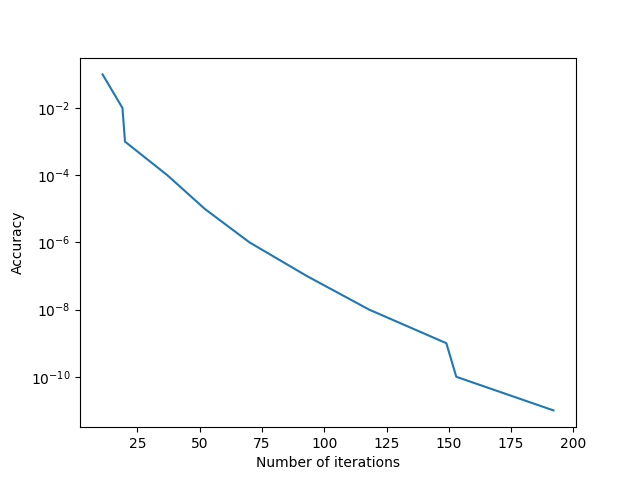
\includegraphics[width=\textwidth]{../results/cg_accuracy.png}
  		\caption{convergence of our problem}
  		\label{cg_acc1}
		\end{subfigure}%
		\begin{subfigure}{.5\textwidth}
 		 \centering
 		 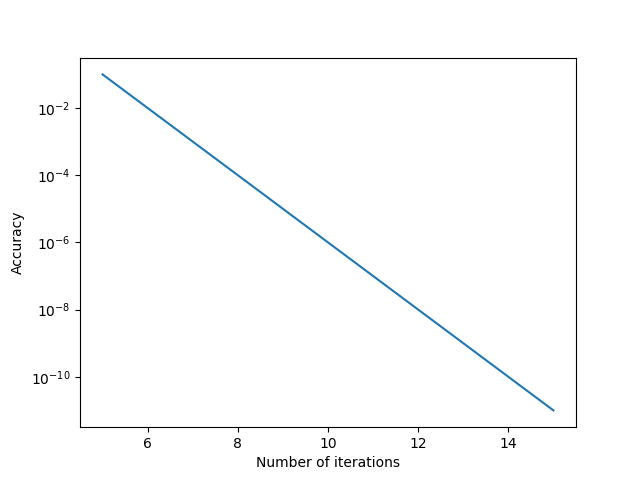
\includegraphics[width=\textwidth]{../results/cg_accuracy_rand.png}
 		 \caption{convergence of a random problem}
 		 \label{cg_acc2}
		\end{subfigure}
		\caption{CG accuracy: number of iterations required to get a specific accuracy value }
		\label{cg_acc}
	\end{figure}
	\begin{figure}
            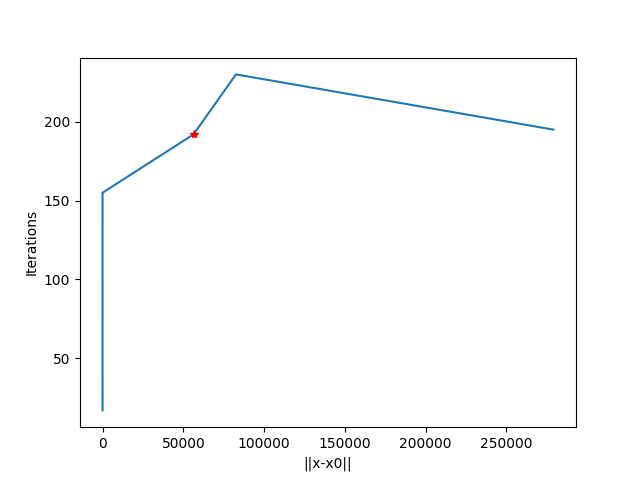
\includegraphics[width=\linewidth]{../results/cg_x0_ite.png}
            \caption{CG with different starting points and with an accuracy of $10^{-11}$. The red star is the 0 vector}
             \label{cg_x0}
       \end{figure}
         \begin{figure}
            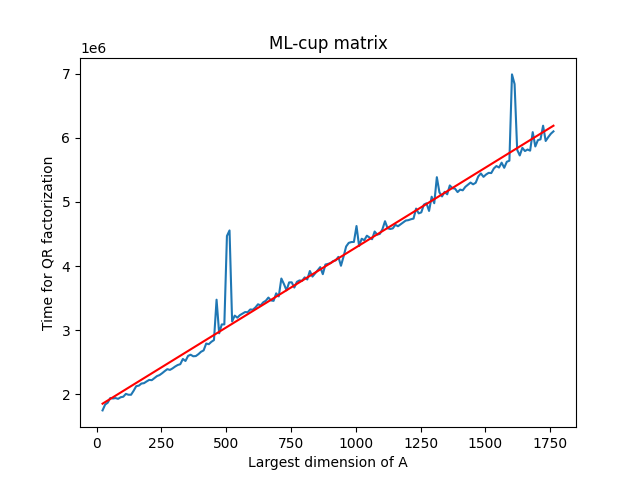
\includegraphics[width=\linewidth]{../results/qr_linear_scaling.png}
            \caption{QR computational time: time required to solve the ML-cup LS problem with the first m rows of A}
             \label{qr_cost}
        \end{figure}
        \begin{figure}
            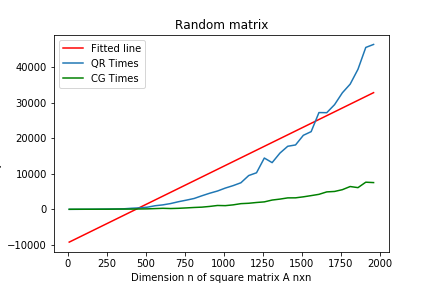
\includegraphics[width=\linewidth]{../results/square.png}
            \caption{QR and CG methods: Computational time w.r.t. dimension n for square matrix $n \times n$}
            \label{square}
        \end{figure}
        \begin{figure}
            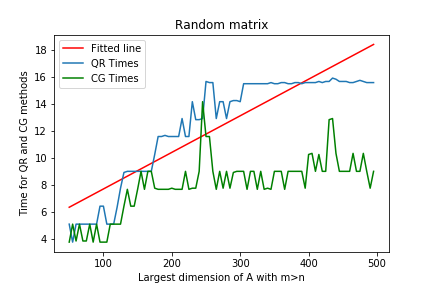
\includegraphics[width=\linewidth]{../results/little_m.png}
            \caption{QR and CG methods: Computational time w.r.t. dimension m for tall thin matrix $m \times n$ with $m > n$}
            \label{little_m}
        \end{figure}
        \begin{figure}
            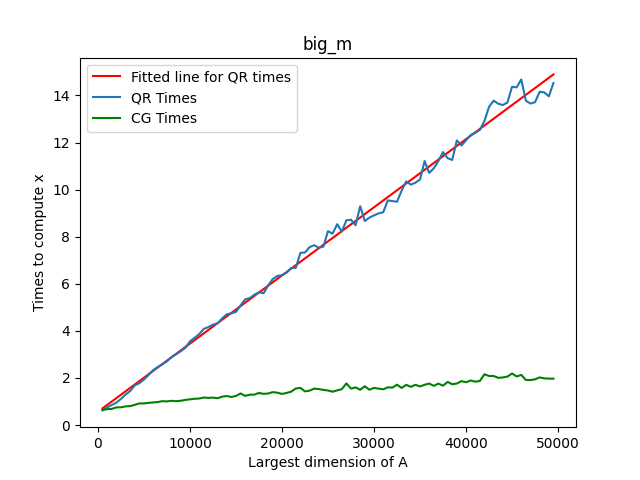
\includegraphics[width=\linewidth]{../results/big_m.png}
            \caption{QR and CG methods: Computational time w.r.t. dimension m for tall thin matrix mxn with $m \gg n$}
            \label{big_m}
        \end{figure}
	


\section{Conclusion}\label{sec:conclusion}
Both QR and CG methods did solve the high conditioned LS problem of ML-cup, but the QR method is two order of magnitude more accurate and, as opposite as CG method, it doesn't require an initial point, a formula for $\beta$ and a number of iteration.
Anyway, the CG method was $\sim 4$ times faster than the QR one, and it is more suitable for large problem because the space it needs is $O(n+m)$ instead of $O(nm)$ ($O(n)$ and $O(n^{2}$) respectively for square matrices). Finally, to reduce the condition number of the problem and hence to get a more accurate result with the CG method, it would be possible to apply the preconditioning technique. 

\bibliography{bibliography}
\bibliographystyle{unsrt}

\end{document}
